% =========================================================
% CHAPTER 2 — STATE OF THE ART
% =========================================================

\chapter{State of the Art}
\label{chap:SoA}

\section{Scope and Methodology}
\label{chap:soa_scope_and_metholodogy}

The aim of this chapter is to review the current literature carried out in the field of T1-Diabetes glycemic prediction. Additionally, different data-balancing techniques proposed for time-series prediction are studied in this section

\subsection{Main Research Areas}
\label{subsec:soa_research_areas}

In order to build a solid state-of-the-art review, this chapter distinguishes between, at least, the following three overlapping but non-equivalent research areas:
\begin{itemize}
    \item T1-Diabetes prediction using CGM data
    \item Data balancing techniques applied to generic machine learning problems and time-series forecasting.
    \item Data balancing approaches for T1 Diabetes prediction
\end{itemize}

\subsection{Literature Search and Selection}
\label{subsec:soa_literature_search}

To perform this review, several academic repositories and scientific databases were consulted, including \textit{Google Scholar \cite{google_scholar}, PubMed \cite{pubmed}, IEEE Xplore \cite{ieee_xplore}, ScienceDirect \cite{sciencedirect}, and SpringerLink \cite{springerlink}.} The search process utilized keywords such as:
\begin{itemize}
    \item \textit{"Type 1 Diabetes}
    \item \textit{"CGM forecasting”}
    \item \textit{"Glycemic prediction”}
    \item \textit{"Data balancing”}
    \item \textit{"Imbalanced regression"}
    \item \textit{"SMOTER"}
    \item \textit{"SMOGN”}
\end{itemize}
The selection of literature was then filtered by its relevance to the scope of this study.

\section{Glycemic Prediction in Type 1 Diabetes}
\label{sec:soa_glycemic_prediction}

\subsection{Evolution of Predictive Architectures}
\label{subsec:soa_prediction_evolution}

Glycemic prediction has recently evolved from simple statistical and physiological approaches towards machine learning. Broad reviews from 2019 \cite{WOLDAREGAY2019109} and 2022 \cite{info:doi/10.2196/34699} state how RNN, SVM, Gaussian and hybrid approaches currently co-exist, while also emphasizing the fact that, for now, there is not an universal model that performs excellently for all clinical contexts.

Recent works \cite{WOLDAREGAY2019109, info:doi/10.2196/34699} follow-up with: LSTM, GRU-based, proposals incorporate attention mechanisms, Transformers and GNN to capture higher complexity.

Furthermore, literature reviews \cite{info:doi/10.2196/34699} state the field has bifurcated into two families: continuous regression of future glucose values and event prediction (primarily hypoglycemia), formulated as a classification problem for early warnings.

\subsection{Prediction Horizons and History Length}
\label{subsec:soa_prediction_horizons_and_history}

The scientific literature \cite{WOLDAREGAY2019109, info:doi/10.2196/34699, s26092675, 10.1371/journal.pone.0253125} converges on the idea that short-medium horizons -- 30 min to 1 hour -- are the most realistic and clinically useful. This range (30 to 60 min horizon) appears consistently in reviews of the T1D prediction literature. Also, evidence shows how the error increases rapidly as this horizon lengthens.

Regarding the length of history window, literature also converges on the idea that most reusable evidence for decision support is concentrated in windows of at least up to one hour before  \cite{WOLDAREGAY2019109, info:doi/10.2196/34699, s26092675, 10.1371/journal.pone.0253125}.

\subsection{Evaluation Metrics and Clinical Taxonomy}
\label{subsec:soa_clinical_metrics}

The evaluation of glycemic prediction requires both statistical and clinical metrics.

Most studies \cite{WOLDAREGAY2019109} in the field use the typical regression problems measures: RMSE, MAE, MSE, etc; since they provide the most direct and uncomplicated numerical estimation of the difference between the predicted and the real values, and allow comparing models in terms of "average numerical accuracy".

However, for problems like this, average error metrics may not be sufficient: a model can obtain a low RMSE while still failing to detect rare but clinically dangerous events. Therefore, these models' evaluation must also consider where the error occurs, not only how large the average error is. For this reason, glucose predicition studies always include additional clinically-oriented metrics. As described in \ref{TIR-explanation}, the standard consensus amongst all literature is "glycemic ranges", often referred as \textbf{Time In Range} \cite{10.2337/dci19-0028}. These metrics are specially relevant for this thesis because they clearly define separate ranges according to their actual clinical relevance, which will allow us to directly quantify the imbalance of the glucose distribution.

Another widely used clinical evaluation tool is the Clarke Error Grid Analysis (CEGA) \cite{10.2337/diacare.10.5.622}. Unlike other generic regression metrics, CEGA not only reflects the numerical difference between the predicted and the real values, but it also classifies those predictions into 5 different categories according to their potential clinical consequences. From safe to critical:
\begin{itemize}
    \item \textbf{Zone A.} Clinically accurate.
    \item \textbf{Zone B.} Slight deviation from ground truth but still clinically safe.
    \item \textbf{Zone C.} Errors that could lead to unnecessary correction.
    \item \textbf{Zone D.} Dangerous failures to detect hypo- or hyperglycemia.
    \item \textbf{Zone E.} Critical errors that lead to the opposite.
\end{itemize}

\begin{figure}[htbp]
    \centering
    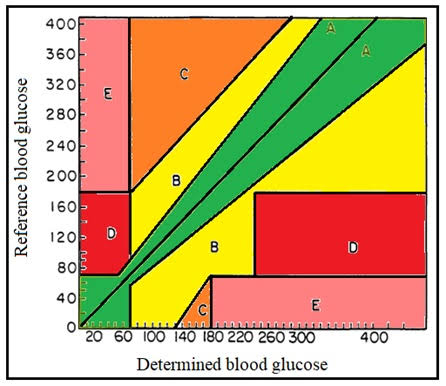
\includegraphics[width=0.75\textwidth]{images/CEGA.jpeg}
    \caption{Clarke Error Grid, classifies glucose predictions according to their clinical risk.}
    \label{fig:clarke-error-grid}
\end{figure}

This taxonomy is particularly important when considering clinical impact: a prediction error in the normo-glycemic may be harmless for the patient, while a similar absoulte error near the critical ranges may dangerously prevent an alarm from being triggered. Therefore, apart from considering numerical regressions errors, a proper model evaluation must also consider this kind of clinical metrics.

Inspired by the Clarke Error Grid, recent research has also studied the possibility of integrating clinical awareness into the learning process itself, through the implementation of \textit{glycemic-aware loss functions}. For example, \textit{\textbf{glucose-specific MSE}} \cite{6135492} extends the traditional MSE by applying higher penalties to clinically harmfull errors. Similarly \textit{\textbf{Hypo-Hyper Loss}} \cite{Darpit2025} introduces asymmetric penalties depending on whether the prediction error affects hypoglycemic or hyperglycemic regions.

\section{Data Balancing in Machine Learning and Time Series}
\label{sec:soa_data_balancing_time_series}

\subsection{Data Balancing in Classification}
\label{subsec:soa_data_balancing_classification}

The problem of data imbalance was first adressed in classification problems. Canonical techniques include the following ones:

\subsubsection{SMOTE}
\label{subsubsec:soa_smote}

\textbf{Synthetic Minority Oversampling Technique} \cite{chawla2002smote}, is an oversampling method used to address class imbalance in classification problems, by generating artificial minority-class instances in the feature space. For each selected minority sample, SMOTE identifies its k-nearest neighbors within the same minority class and creates a new synthetic sample by linear interpolation between the original point and one randomly chosen neighbor. The new instance is randomly generated along the segment connecting both samples. While naive duplication of samples would only increase density inside the minority class, this approach introduces more diversity to the group, helping the classifier learn a less biased decision boundary toward the majority class.

\subsubsection{Borderline-SMOTE}
\label{subsubsec:soa_borderline_smote}

\textbf{Borderline-SMOTE} \cite{10.1007/11538059_91} is an extension of SMOTE that also generates synthetic samples, but only around the minority-class instances that are located near the decision boundary, where misclassification is more likely. Synthetic examples are then created by interpolating between these "borderline" instances and their minority-class neighbors. This approach makes the oversampling process focus on the most informative and vulnerable regions of the feature space, helping the classifier perform better near the boundaries.

\subsubsection{ADASYN}
\label{subsubsec:soa_adasyn}

\textbf{Adaptive Synthetic Sampling} \cite{4633969} is an oversampling technique that addresses data balancing by focusing on areas where learning is harder. Like SMOTE, ADASYN generates synthetic samples via interpolation between minority-class near neighbors. However, ADASYN "adaptively" assigns a higher number of synthetic samples to those minority instances that are surrounded by more majority-class neighbors, since these points are the most difficult to classify.

\subsection{Balancing Methods for Regression}
\label{subsec:soa_data_balancing_regression}

In regression, the situation is more complex because discrete boundaries do not exist. There is no such thing as "rare regions" because all the points are inherently considered to be equally important. This differentiation is key, and directly answers why data-balancing in regression has historically been treated much less than in classification. However, some extensions of the previous techniques have arisen from this same concern:

\subsubsection{SMOTE-R}
\label{subsubsec:soa_smoter}

\textbf{SMOTE for Regression} \cite{10.1007/978-3-642-40669-0_33}, is an extension of SMOTE for imbalanced regression problems, where the target variable is continuous rather than categorical. Instead of oversampling a minority class, SMOTE-R focuses on rare or highly relevant target-value "regions" – such as extreme glucose values in this case. Like SMOTE, it generates synthetic samples by interpolating between near neighbors, but determines which areas should be oversampled according to their relevance of the continuous target.

\subsubsection{SMOGN}
\label{subsubsec:soa_smogn}

\textbf{Synthetic Minority Oversampling Technique for Regression with Gaussian Noise} \cite{pmlr-v74-branco17a}, is an extension of SMOTE-R that generates synthetic samples in highly relevant target regions by combining simple interpolation with the addition of Gaussian noise. This makes the generated data more diverse and helps to avoid the limitations of simple interpolation in cases where rare regions are irregularly distributed.

\vspace{1em}

Recent works has arisen other -- while much less adopted in the literature -- data balancing techniques such as: \textbf{SERA} \cite{5178874}, which evaluates regression error by giving greater importance to rare or highly relevant target values; \textbf{Balanced MSE} \cite{Ren_2022_CVPR}, which extends MSE to reduce of highly-frequent target values during training; and \textbf{Geometric variants} \cite{CAMACHO2022116387}, which redefine the synthetic samples generation to consider the geometric distribution of the local area instead of simple interpolation.

\section{Data Balancing Applied to Glycemic Prediction}
\label{sec:soa_data_balanding_glycemic_prediction}
The importance of this job does not lie on studying glycemic prediction and data-balancing techniques separately, but on identifying what have been done in combination of both, to improve model behavior in rare but clinically critical glycemic regions.

\subsection{Prevalence of Explicit Balancing}
\label{subsec:soa_data_balancing_prevalence}

When narrowing the scientific research to the combined focus of this thesis, explicit balancing appears much less than expected in glycemic predicion studies. Literature reviews \cite{info:doi/10.2196/34699} can mostly be catogorized into two big areas: glucose prediction and event prediction; but balancing the continous target is hardly ever considered the central theme.

\subsection{Previous Oversampling Approaches}
\label{subsec:soa_oversampling_approaches}

Mayo et. al \cite{10.1371/journal.pone.0225613} author one of the only -- if not the only -- studies that uses “glycemic-aware” metrics and oversampling techniques for predicting blood glucose. They demonstrate two important things: first, that the best model highly depends on the glycemic sub-range, there is not a model that performs well for all; and second, that oversampling helps improving prediction performance specifically in hypoglycemia. 

Mayo et al. use Random Oversampling, SMOTE, and ADASYN, to generate synthetic samples for the minority ranges. In their results, an MLP (Multi-Layer Perceptron) trained with the oversampled data was the best option for the hypoglycemic range, while a linear SVR (Support Vector Regression) performed better in the normal and hyperglycemic ranges.

\subsection{Synthetic Data Using Generative Models}
\label{subsec:soa_over_sampling_gnn}

In this other work by Nogher et. al \cite{s22134944}, they explore the possibility of using generative deep learning-based architectures to generate synthetic data. This idea arises from the conception that traditional mathematical generators often fail to accurately replicate the complex, individualized physiological behaviors of real patients.

In their results, they demonstrate that training models with datasets that have been synthetically oversampled with the mentioned mechanisms, achieves a general improvement across all evaluated metrics. This work sets the precedent in the use of generative machine learning techniques to train glucose prediction model.

\subsection{Patient Heterogeneity as a Contextual Factor}
\label{subsec:soa_patient_heterogeneity}

While not directly relevant to the scope of this thesis, it also interesting to consider other related literature that shows that patient characteristics -- such as age, gender, or comorbidities --  may affect the frequency and predictability of different glycemic ranges. Recent research has explored the role of patient heterogeneity in glucose prediction. Baños, Villalonga et al. \cite{10.1007/978-3-032-02725-2_51} studied the impact of factors such as age, gender, hypertension, obesity, and hypothyroidism on the performance of Linear, LSTM, and CNN models using the T1DiabetesGranada dataset. Their results showed that incorporating patient-specific factors can improve prediction accuracy, particularly for elderly patients and those with hypertension or obesity.

\section{Synthesis and Research Gap}
\label{sec:research_gap}

\subsection{Summary of the State of the Art}
\label{subsec:soa_summary}

The literature review performed in this chapter clearly shows how previous works have extensively studied studied glucose forecasting, event prediction, clinical evaluation metrics, and different forms of data augmentation or oversampling. However, it also shows that most glucose prediction models are still being evaluated through typical regression global error metrics, which may be hiding important clinical risks.

\subsection{Identified Research Gap}
\label{subsec:research_gap}

Although previous studies have separately explored glucose forecasting, clinical metrics, and data-balancing mechanisms, there is still limited evidence on whether balancing the training data according to glycemic ranges proportions can improve model performance in underrepresented but clinically-critical regions.

Therefore, the gap addressed in this thesis can be formulated through the following question: \textbf{can data-balancing techniques -- such as SMOTER, SMOGN, or related approaches -- improve predictive performance across imbalanced glycemic regions without substantially degrading overall accuracy?}. This study investigates this hypothesis and evaluates its validity.

In order to address this question, this thesis will analyze the distribution of glucose values in three CGM datasets (DiaTrend, REPLACE-BG and T1DiabetesGranada), \textbf{apply balancing techniques according to clinically defined glycemic ranges}, train existing predictive models under controlled experimental conditions, and compare their performance statistically.
